\documentclass[preprint,10pt,authoryear]{elsarticle}

%% Use the option review to obtain double line spacing
%% \documentclass[preprint,review,12pt]{elsarticle}

%% Use the options 1p,twocolumn; 3p; 3p,twocolumn; 5p; or 5p,twocolumn
%% for a journal layout:
%% \documentclass[final,1p,times]{elsarticle}
%% \documentclass[final,1p,times,twocolumn]{elsarticle}
%% \documentclass[final,3p,times]{elsarticle}
%% \documentclass[final,3p,times,twocolumn]{elsarticle}
%% \documentclass[final,5p,times]{elsarticle}
%% \documentclass[final,5p,times,twocolumn]{elsarticle}

%% if you use PostScript figures in your article

%% or use the graphicx package for more complicated commands
\usepackage{graphicx}
%% or use the epsfig package if you prefer to use the old commands
\usepackage{epsfig}

%% The amssymb package provides various useful mathematical symbols
\usepackage{amssymb,amsmath}
%% The amsthm package provides extended theorem environments
%% \usepackage{amsthm}

%% The lineno packages adds line numbers. Start line numbering with
%% \begin{linenumbers}, end it with \end{linenumbers}. Or switch it on
%% for the whole article with \linenumbers after \end{frontmatter}.
\usepackage{lineno}

%% natbib.sty is loaded by default. However, natbib options can be
%% provided with \biboptions{...} command. Following options are
%% valid:

%%   round  -  round parentheses are used (default)
%%   square -  square brackets are used   [option]
%%   curly  -  curly braces are used      {option}
%%   angle  -  angle brackets are used    <option>
%%   semicolon  -  multiple citations separated by semi-colon
%%   colon  - same as semicolon, an earlier confusion
%%   comma  -  separated by comma
%%   numbers-  selects numerical citations
%%   super  -  numerical citations as superscripts
%%   sort   -  sorts multiple citations according to order in ref. list
%%   sort&compress   -  like sort, but also compresses numerical citations
%%   compress - compresses without sorting
%%
%% \biboptions{comma,round}

% \biboptions{}
\usepackage{hyperref}
\usepackage{color}
\usepackage{textcomp}
\usepackage{multirow}
\usepackage{float}

\journal{Computer and Chemical Engineering}

\begin{document}

\begin{frontmatter}
\title{Accelerating multi-dimensional population balance model simulations using GPU with a highly scalable framework.}


\author[label1]{Chaitanya Sampat}
\author[label1]{Yukteshwar Baranwal}
\address[label1]{Chemical and Biochemical Engineering, Rutgers University, Piscataway, NJ, USA - 08854}
\author[label1]{Rohit Ramachandran\corref{cor1}}
\ead{rohitrr@soemail.rutgers.com}
\cortext[cor1]{Corresponding author}
%\ead[url]{pslrutgers.com}

\begin{abstract}
Population Balance models are widely used in pharmaceutical industry to simulate
and optimize the granulation process.Prediction of the distribution of many 
particulate sytems with the evolution of time using these models, has become an 
efficient tool for the on-line control of the granulation process. 
With increase in the number of components and phases in a particulate mixture, 
complexity of PBM increases. This leads to multi-dimensional matrix calculations 
requiring great computational power. Over the past decade, graphical process 
units (GPUs) are increasingly being used for computation. This study focuses on the 
development of an algorithm to parallelize the various nested loops inside the PBM. 
The PBM was developed for a continuous high shear granulation process and was made 
specifically for NVIDIA GPUs as it was developed on CUDA C/C++. The communication 
time is much lower in comparison to the speedup achieved in the parallel section 
of the code on the GPUs. The speed up achieved was significant compared to the PBM 
code when run in serial or in on multi-core configuration. The speed improvements 
for the code was reported for various CPU \& GPU architectures and configurations. 
The speed improvements were also tested with various combinations in 
discretization of the granulator geometry and threads used for calculations. 
\end{abstract}

\begin{keyword}
%% keywords here, in the form: keyword \sep keyword
Population Balance Model \sep GPU \sep Paralllel Computing \sep Granulation \sep MPI
%% MSC codes here, in the form: \MSC code \sep code
%% or \MSC[2008] code \sep code (2000 is the default)
\end{keyword}

\end{frontmatter}

\begin{linenumbers}
%% main text
\section{Introduction}
\label{secIntro}
Various chemical industries like detergent, food, pharmacuetical, fertilizers, 
catalyst encounter particulate processing daily. These processes 
constitute to about 50\% of the world's chemical production \citep{seville1997}. 
In the pharmacuetical industry, particulate processes are widely used to increase 
the size of the granules, improve flowability, increase yield strength etc. One of 
major processes in amoing these to increase the granule size is granulation. 
Granulation is the process in which fine pharmacuetical powder 
blends are converted to larger granules using a liquid or a dry binder \citep{Chaturbedi2017}. 
These larger granules help in better flow ability and strength to these mixtures 
aiding further processing. 

%Due to the large number of collisions inside these systems, modeling these systems is a challenge.

Understanding the dynamics of the continuous granulating system is vital for its smooth 
operation and to reduce the amount of waste generated in the development phase. The Food 
and Drug administration (FDA) has also been promoting a similar initiative with its 
Quality by Design (QbD) and Process Analytical Tools (PAT) principles~\citep{sen2014}. 
Thus, a process model for the system becomes an integral part of the development phase. 
A model which predicts the bulk mechanical properties of the mixture as well as a particle size 
distribution (PSD) is required. Over the past decade, Population Balance Models (PBMs) have been used 
to predict the behaviour of granulation processes \citep{Barrasso2013},\citep{Ramachandran2009}. 

PBMs are used to calculate bulk rate processes ocurring during granulation. PBMs are sometimes 
unable to integrate certain information, thus a mechanistic kernel can be 
introduced in these models to make them more accurate. Another way to increase its accuracy, 
is to incorporate larger number of solid bins inside the PBM. The increase in the number of 
solid bins leads to an increase in calculations for each time step, leading to a higher 
simulation times. The calculations increase by a factor of $2^n$ where n being the number 
of solid bins. An accurate model which incorporates higher number of solid bins as well as 
includes a mechanistic kernel in its calculations is expected to be very 
slow to simulate and could take upto hours to complete. Such models and their solving 
techniques are not viable to be used in real time sytem control. Thus, there is a need to 
solve these models quicker.

The advancement of computers and its peripherals in recent years have led to a great increase in 
computational resources leading to faster simulations. The recent central processing unit (CPU) 
now contains various of cores thus making it possible to run multiples processes in parallel. 
In order to take advantege of a highly parallel framework, large number of cores are needed 
which may not be possible in a personal desktop and a supercomputer cluster needs to be used.
Another computer peripheral that can to be used to run a highly parallel code is the computer's 
graphic processing unit (GPU)~\citep{Prakash2013b}. These GPUs contain thousands of compute 
cores that can be used run tasks in parallel. Thus, a desktop equipped with a GPU could 
compute the same results as a CPU code on supercomputers in lesser amount of time as seen in Section \ref{secResults}.
With the launch of Compute Unified Device Architecture (CUDA), NVIDIA made it easier to use GPUs for 
general parallel programming in an approach usually termed as general purpose computing on GPUs (GPGPUs).

In the present study, a mechanistic multi-dimensional PBM was developed such that it was not 
only accurate but also scalable since the number of solid bins could be changed to alter its 
behaviour. This model was developed in C++ to be run on CPUs. This C++ model was parallelised 
using Message Parsing Interace (MPI) which is parallel application programming interface (API). 
This model was developed NVIDIA GPUs and was parallelized using the CUDA toolkit. The timings of 
the simulations were then compared for each of these cases. The scalability of the GPU based code 
was also tested to obtain speed improvements over serial CPU code.


\section{Background and previous works}
\label{secBkgd}
\subsection{Granulation and population balance modeling}
Granulation is the process of engineering granules from pharmacuetical powder blends 
with the addition of liquid or solid binders. This process is usually carried out 
to obtain granules with a certain PSD,  bulk densities and other physical properties~\citep{Barrasso2015cerd}.
There are about 3 rate processes that occur due the addition of a liquid binder to the 
powder mixture are wetting and nucleation, consolidation and aggregation, and breakage 
and attrition~\citep{sen2014}. In a high shear granulator, the particles are rendered wet 
when they come in contact with the liquid binder, which also aids in granule formation due to 
liquid bridges. These granules can also break into smaller fragments due to shear stresses, 
compressive and tensile forces that are exerted on to the system due the impeller, 
particle-particle interactions and particle-wall interactions.

To understand the process dynamics and control these process, population balance equations 
have been accepted as a relevant methodology \citep{Immanuel2005}. Population balances have been successful in 
predicting physical phenomena occuring in granulation such as aggreagation, breakage and 
consolidation. These models preidct how groups of distinct entities inside the pharmacuetical 
powder behave on a bulk scale due to process parameters over time of granulation. A
general representation of the model is:

\begin{align}
\frac{ \partial}{\partial t}&F(\textbf{v},\textbf{x},t) + \frac{\partial}{\partial 
\textbf{v}}[F(\textbf{v},\textbf{x},t)\frac{d\textbf{v}}{dt}(\textbf{v},\textbf{x},t)] 
+ \frac{\partial}{\partial \textbf{x}}[F(\textbf{v},\textbf{x},t)\frac{d\textbf{x}}{dt}
(\textbf{v},\textbf{x},t)] \notag\\
    &= 
\Re_{formation}(\textbf{v},\textbf{x},t)+\Re_{depletion}(\textbf{v},\textbf{x},t)
+\dot{F}_{in}(\textbf{v},\textbf{x},t) -\dot{F}_{out}(\textbf{v},\textbf{x},t) 
\label{eqn:bkgd_pbm_general} 
\end{align}

where $\textbf{v}$ is a vector of internal 
coordinates.  $\textbf{v}$ is commonly used to describe the solid, liquid, 
and gas content of each type of particle. The vector $\textbf{x}$ represents 
external coordinates, usually spatial variance. $F$ represents the 
number of particles present inside the system, $\dot{F}_{in}$ 
and $\dot{F}_{out}$ is the rate of particles coming in and going out the 
system respectively. $\Re_{formation}$ and $\Re_{depletion}$ are the rate of 
formation and depletion due various phenomena occuring in granulation. 

Prediction of PSDs and other particle bulk properties is highly dependent on 
the kernels used to describe the sub-processes inside granulation. Identification 
of a kernel that describes the sub-processes suitably is of the essence in this model 
since they are not only size dependent but also time dependent. Recently, various 
mechanistic kernels have been developed that help capture the micro-mechanics of the 
system, which help in better prediction of the final particle size \citep{Barrasso2015processes}. 
Several of these kernels maybe dependent on other physical simulations such as Discrete 
Element Model (DEM) to obtain certain information about the microscopic phenomena 
occuring inside the system.


\subsection{Parallel Computing}
Computing with its current infrastructure has become a very important tool in sciece. 
Paralllel computing is one of most extensively used type of computing used by scientists 
to perform simulations. It is the process of splitting of larger calculations into 
many smaller processes executed concurrently \citep{Almasi1989}. This type of execution 
helps achieve large speed gains overs simulations run on a single core in a serial manner.
The computational task can be decomposed by various means to help simulate the system 
in a reasonable amount of time. The simulation problem can be decomposed either 
at the task level or at the data level. Task parallelism involves each process to 
behave distinctively from another as they would each be performing different operations. 
These multiple operations could be performed on a single data set or on multiple data 
sets, known as multiple instruction single data (MISD) and multiple instruction 
multiple data (MIMD) respectively. On the other hand, data parallelism 
involves the distribution of data across various processes which usually perform same set of 
operations on the data \citep{solihin2015}. This type of parallelism is also known 
as single instruction multiple data (SIMD). These two types of parallelism can also 
be combined in certain systems, thus decreasing the simulation times further.

\subsection{GPU based parallel computing}
Tradionally, large parallel jobs needed to be run on supercomputers which had thousands 
of cores, but these are require special components making them expensive.
Graphic processing unit (GPU) were initally mainly used for vector calculations to support 
graphics inside a computer system. But, lately GPU manufacturers have started to promote them 
general computing as well. This form of computing has been gaining popularity among scientists 
to accelerate simulations \citep{kandrot2011}. These GPUs dominantly have a 
massively parallel architecture with hundreds to thousands of computational cores 
which can thousands of active threads simulataneously \citep{keckler2011}. 
Modern GPU computing can be exploited using parallel programming languages 
such as OpenCL and CUDA. 

CUDA is an application programming interface (API) developed by NVIDIA \citep{NVIDIA2012} that enables 
users to program parallel code for execution on the GPU. This is framework is an 
extension implemented on top of C/C++ or Fortran. Parallel code for the GPU is written 
as kernels, which theoritically are similar to functions or methods in traditional 
programming languages. Only few sections of the code can be written in terms of kernel 
while the remaining has to be executed in serial on the CPU of the system. The \texttt{nvcc} 
compiler from the CUDA toolkit prioritizes the compilation of these kernels before 
passing the serial section of the code to the native C/C++ compiler inside the system. 
There are three main parallel abstractions that exist in CUDA are grids, blocks and 
threads \citep{santos2013}. Each CUDA kernel is executed serially during the execution 
of the program unless specified, where the kernels can be run in parallel using CUDA 
streams. Each kernel executes as a grid which in turn consists of various blocks which 
are consistuted by various threads. This thread-block-grid hierarchy helps obtain fine 
grained data level and thread level parallelism. An illustration of this hierarchy is 
observed in Figure \ref{fig:bkg_gpu_arch}.

Another important aspect related to GPU parallelization is the data communication between the threads. 
The GPU consists of various memory modules with different access limitations as shown in Figure 
\ref{fig:bkg_gpu_arch}. The threads inside each block can communicate with each other using the 
shared memory. This memory is local to the block where these threads exist i.e. they are not 
accessible by threads from other blocks. In addition to the shared memory each thread has its 
own local memory where local/temporary variables for each kernel can be saved to them. 
The threads from different communicate with each other using the global memory which is visible to 
all blocks inside the GPU at the cost of higher communication times. Accessing of data from the 
local memory is the fastest for a thread and its slows down as we move towards shared block memory 
and the least for accessing data from the global GPU memory. 


\begin{figure}
\centering
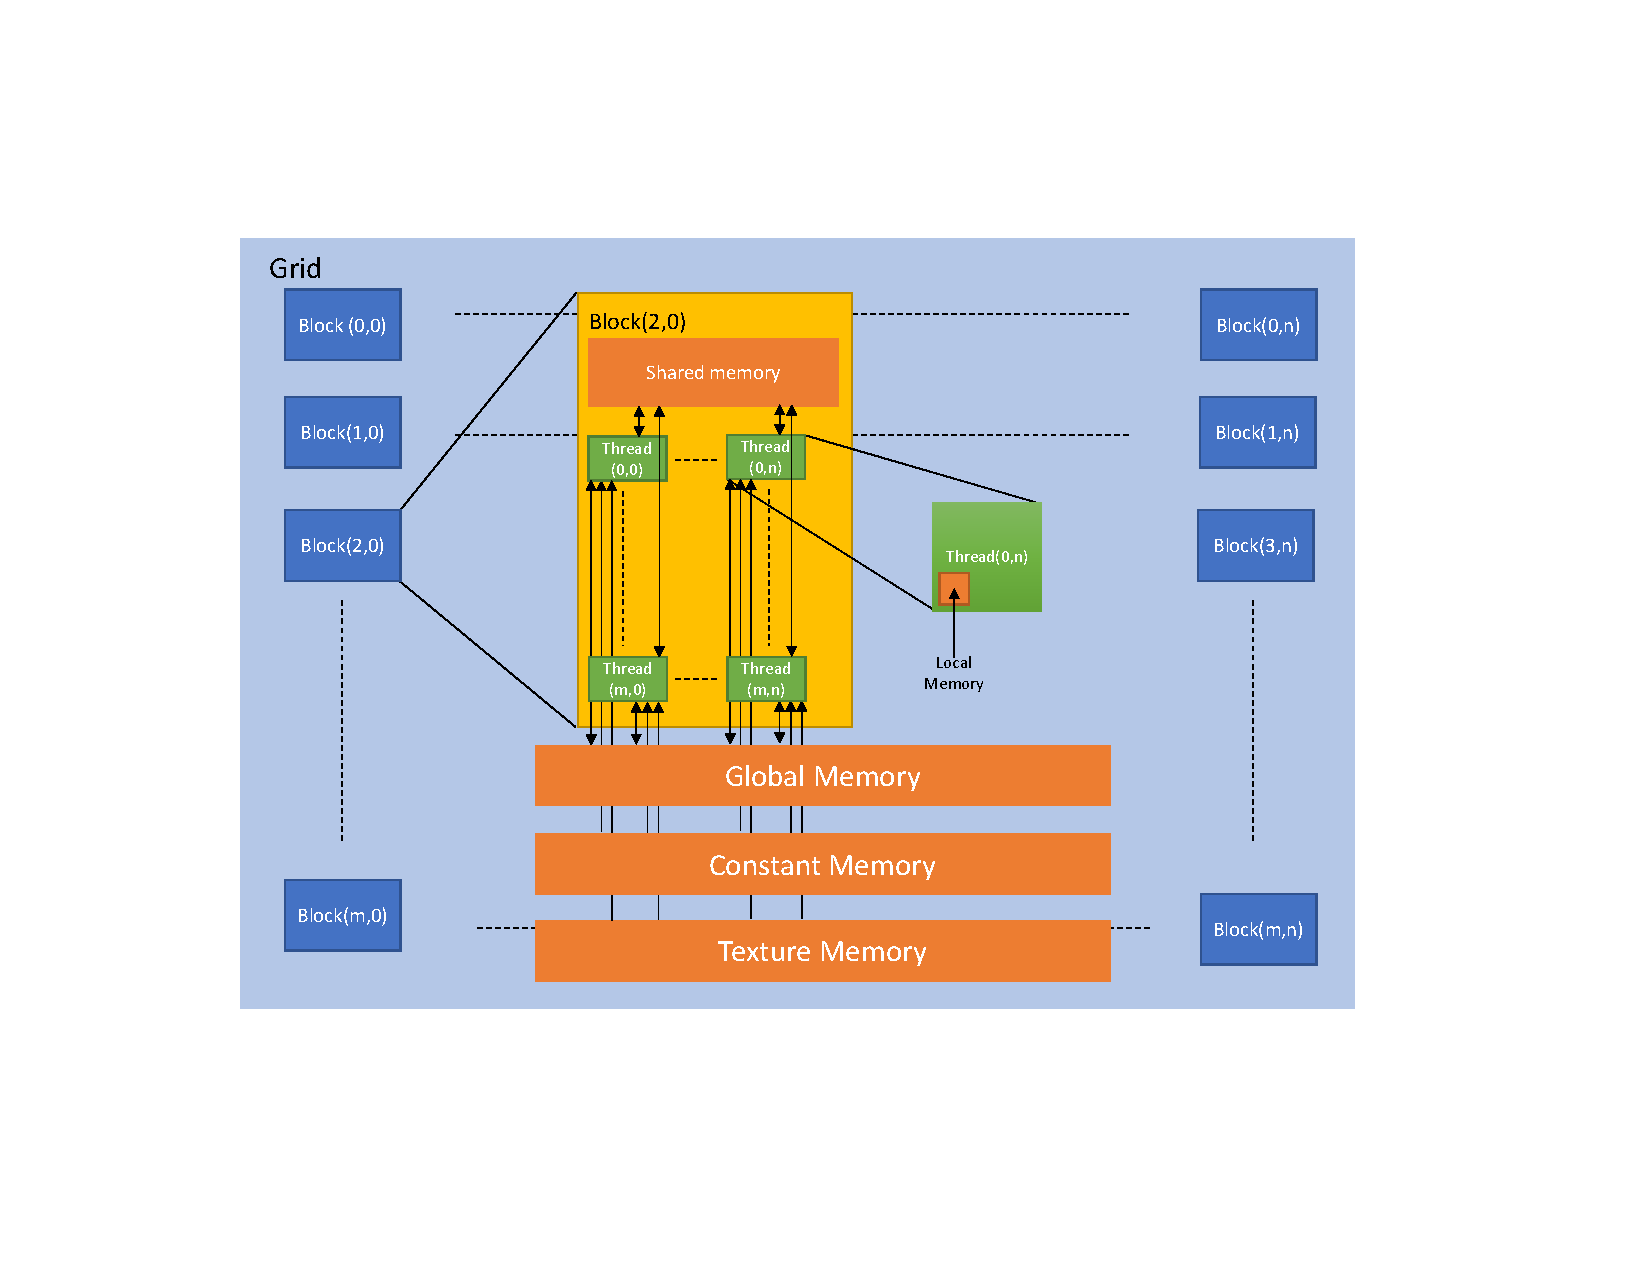
\includegraphics[scale=0.6]{bkg_gpu_arch.pdf}
\caption{The parallel structure matrix inside the GPU and the various memories associated 
with each structure.}
\label{fig:bkg_gpu_arch}
\end{figure}


\subsection{Previous parallel PBM works}
PBMs have known to be been computationally intensive especially ones with larger internal 
coordinates and higher dimensions. Thus, several researchers have made attempts to increase 
the speed of these simulations. \cite{Gunawan2008} developed a parallelization technique 
for a high-resolution fininte volume solution of the PBM. The parallel algorithm presented by 
\cite{Gunawan2008} in their scale up studies for the PBM upto 100 cores achievd good 
parallel efficiencies, implying the algorithm's effectiveness. The study was not performed for 
higher number of dimensions inside the PBM. This study also suggested that an algorithm 
with a shared memory model could help improve simulation speeds further. A hybrid memory model 
was implemented by \cite{Bettencourt2017} to obtain speed improvements of about 98\% from the 
serial code. This implementation took into account both Message Parsing Interface (MPI) as well 
as Open Multi-processing (OMP). A similar PBM parallelization approach was also undertaken in 
\textcolor{red}{cite CDSE} and a speed up of about 13 was obtained. 

Algorithms to parallelize the PBM codes on GPU have been studied briefly by \cite{Prakash2013b} 
using the inbuilt MATLAB's parallel computing toolbox (PCT). This study was able to achieve 
good speed ups but could have been higher if the code had been implemented in native programming 
languages such as C or FORTRAN. Other works that have used GPU acceleration to improve computation 
times for their population balance simulations include those from various other chemical engineering 
processes such as crystallization \citep{Szilagy2016}, combustion \citep{Shi2012}, multiphase flow 
\citep{santos2013}, coagulation dynamics \citep{Xu2015}


cite cdse, Santos, Gunuwan and other from CDSE
cite Nagy, Santos, Green etc for the PBM GPU part

\section{Method and implementation}
\label{secMethods}
\subsection{PBM implementation}
relate each equation of the PBM used to each process and explain a bit
\subsection{MPI implementation}
elaborate how the geometry was divided into compartments and how each \\
compartment was sent to each block
\subsection{GPU implementation}
Elaborate how each block was each compartment and how each thread was 
parallelized to perform calculation for solid 1 solid 2 combination.

\section{Results and discussions}
\label{secResults}

\section{Conclusions}
\label{secConc}
\end{linenumbers}

\bibliographystyle{elsarticle-harv}
\bibliography{pbmGpuPaper}


\end{document}

%%
%% End of file `elsarticle-template-num.tex'.
